\documentclass{standalone}

\renewcommand{\familydefault}{\sfdefault}
\usepackage{amsmath}
\usepackage{tikz}
\usetikzlibrary{arrows.meta, positioning, calc, }

\newcommand{\quadrup}[5]{%
  % #1 = x, #2 = y, #3 = largura, #4 = altura, #5 = cor
  \fill[#5]
    (#1-0.5*#3,#2+0.5*#4) --
    (#1,#2) --
    (#1+0.5*#3,#2+0.5*#4) --
    cycle;
  \fill[#5]
    (#1-0.5*#3,#2-0.5*#4) --
    (#1,#2) --
    (#1+0.5*#3,#2-0.5*#4) --
    cycle;
}

\newcommand{\bpmrule}[4]{%
  % #1 = x_inicial, #2 = altura total H, #3 = número de marcas, #4 = cor
  \draw[#4, thick] (#1,-0.5*#2) -- (#1,0.5*#2);
  \foreach \x in {1,...,#3} {
    \pgfmathparse{\x == 33 ? 1 : 0}
    \ifnum\pgfmathresult>0\relax
      \draw[#4, thick] (#1, 0.5*#2 - #2*\x/#3 + 0.5*#2/#3)
                    -- ++(0.2,0) node[right, xshift={-0.25em}] {\footnotesize 0};
    \else
      \pgfmathparse{mod(\x - 3,5) == 0 ? 1 : 0}
      \ifnum\pgfmathresult>0\relax
        \draw[#4, thick] (#1, 0.5*#2 - #2*\x/#3 + 0.5*#2/#3)
                    -- ++(0.2,0);
      \else
        \draw[#4, line width=0.65pt] (#1, 0.5*#2 - #2*\x/#3 + 0.5*#2/#3)
                      -- ++(0.1,0);
      \fi
    \fi
  }
}

\begin{document}

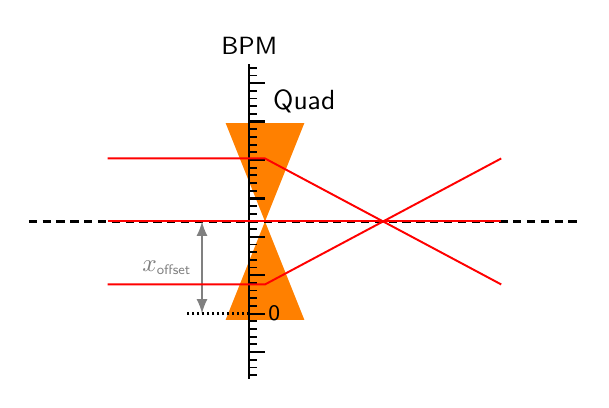
\begin{tikzpicture}[>=latex]

    \pgfmathsetmacro{\dy}{0.8}   
    \coordinate (O) at  (0, 0);
    \coordinate (Op) at (0, \dy);
    \coordinate (Om) at (0, -\dy);

    \coordinate (S) at  (-2, 0);
    \coordinate (Sp) at (-2, \dy);
    \coordinate (Sm) at (-2, -\dy);

    \coordinate (F) at  (3, 0);
    \coordinate (Fp) at (3, -\dy);
    \coordinate (Fm) at (3, \dy);

    \pgfmathsetmacro{\qlarg}{1}   
    \pgfmathsetmacro{\qalt}{2.5}

    \quadrup{0}{0}{\qlarg}{\qalt}{orange}

    \node[above] at ($(O)+(0.5,\qalt/2)$) {Quad};
    
    \draw[thick, densely dashed] (-3, 0) -- (4, 0);

    \pgfmathsetmacro{\sbpm}{-0.2}
    \bpmrule{\sbpm}{4}{41}{black}
    \pgfmathsetmacro{\dybba}{-1.17}
    \pgfmathsetmacro{\xbpm}{0.1}
    \node[above, black] at (\sbpm, 2) {\small{BPM}};
    \draw[thick, gray, <->] (\sbpm-0.6, \dybba) -- (\sbpm-0.6, 0) node[midway, left] {\small $x_\text{\tiny{offset}}$};
    % \draw[thick, gray, <->] (\sbpm-1.5, \dybba) -- (\sbpm-1.5, \xbpm) node[midway, left, yshift={-0.5em}] {\small $x_\text{\tiny{offset,BBA}}$};
    % \draw[thick, densely dotted, black] (\sbpm, \xbpm) -- ++(-1.6, 0);
    \draw[thick, densely dotted, black] (\sbpm, \dybba) -- ++(-0.8, 0);

    \draw[line width=0.7pt, red] (S) -- (O) -- (F);
    \draw[line width=0.7pt, red] (Sp) -- (Op) -- (Fp);
    \draw[line width=0.7pt, red] (Sm) -- (Om) -- (Fm);

\end{tikzpicture}


\end{document}
